\documentclass[12pt,a4paper]{article} 

\usepackage{float,times,graphicx,mathtools}
\usepackage{amsmath}
\usepackage{amsfonts}
\usepackage{amssymb}
\usepackage{latexsym}
\usepackage{epsfig}
\usepackage{graphicx}
\usepackage{caption}
\usepackage{subcaption}
\usepackage{color}
\usepackage{pdfpages}
\usepackage{natbib}
\usepackage[space]{grffile}
\usepackage{wrapfig}
\usepackage{subcaption}
\usepackage{url}
\usepackage{bbm}
\usepackage{tikzsymbols}

\DeclareMathOperator{\logit}{logit}
\DeclareMathOperator{\tr}{tr}
\bibpunct[, ]{(}{)}{;}{a}{,}{,}
\graphicspath{{../Burkina Faso/12/}}  
\addtolength{\oddsidemargin}{-1in}
	\addtolength{\evensidemargin}{-1in}
	\addtolength{\textwidth}{1.75in}
	\addtolength{\topmargin}{-1.3in}
	\addtolength{\textheight}{2in}
\date{\vspace{-5ex}}

\begin{document}
\begin{itemize}
\item I have tried to use a half-Normal prior on the "standard deviation" of the spline coefficients, $\lambda^{-1/2}$, but it failed to converge even for Zimbabwe

\item all hyperpriors are now common between sexes, except for the dispersion parameters for the Negative Binomial (maybe will fix that too)

\item simulating the posterior of the hyperparameters took extremely long time, given up on that at the moment

\item Explored the PC priors and trimmed down the number of hyperparameters, as well as added spikes for TiPS at 5 and 10 that were previously missing, will add plots visualising the marginal prior distribution of the parameters soon (at the moment fitting the gumbel too all countries and don't want R to explode)
	\begin{itemize}
	\item[--]  For the mortality model parameters, these are previously given GMRF with precision matrix $\boldsymbol{Q} = \lambda_1 (\boldsymbol{{D_2}'{D_2}} + \lambda_2 \boldsymbol{I})$. The ratio between $\lambda_1$ and $\lambda_2$ controls how much the linear extrapolation is shrunk towards 0. Writing the penalty (precision matrix) as $\boldsymbol{Q} = \tau (\boldsymbol{{D_2}'{D_2}} + c \boldsymbol{I}) = \tau \boldsymbol{R}$, under the PC priors, we elicit information on the effective degrees of freedom (EDF) and translate this into a prior for $\lambda$. Following Ventrucci and Rue (2016), the EDF is approximated by the trace of the hat matrix under the classical linear regression model. Consider:
	\begin{align*}
	 \boldsymbol{y} &= \boldsymbol{B \beta} + \boldsymbol{\varepsilon} \\
	\text{where} \quad \varepsilon &\sim N(0, \tau_{\varepsilon}^{-1}) \\
	\text{with penalty} \quad   &\tau \boldsymbol{\beta'R\beta},
	\end{align*}
the hat matrix is $(\boldsymbol{B'B} + \frac{\tau}{\tau_{\varepsilon}}\boldsymbol{R})^{-1}\boldsymbol{B'B}$ and hence the EDF is $d(\tau) = tr(\boldsymbol{I} + \frac{\tau}{\tau_{\varepsilon}}\boldsymbol{R(B'B)}^{-1})^{-1} = \sum_k (1 + \frac{\tau}{\tau_{\varepsilon}} v_k) ^{-1}$. By setting a upper bound of the EDF $U$ such that $P(d > U) = \alpha$ for some small probability $\alpha$, the PC prior for $\tau$ can be obtained as a Gumbel Type 2 $(\frac{1}{2}, \theta)$ where $\theta = -\log(\alpha) \sqrt{d^{-1}(U)}$.

There are several tuning parameters for this PC hyperprior, $\alpha, U, \tau_{\varepsilon}$ and $c$. I set $\alpha = 0.01$ and $U = 1$ for $\{\phi, A\}$, $U = 1.5$ for $\{\psi, B\}$ and $U = 5$ for $\{\lambda, \delta, \epsilon \}$, meaning that we don't really believe the EDF of the splines would be higher than 1, 1.5 or 5 for the respective parameters, which correspond to a constant ($U = 1$) and somewhere between a constant and a linear trend ($U = 1.5$). 

$c$ is also estimated as a parameter but now I have decided to fix it as a constant to remove the computational burden. A higher value of $c$ allows a lower $\tau$ in order to reach a specific EDF. In the limiting case when $c \to \infty$, the penalty degenerates to a i.i.d precision matrix. Conventionally in Bayesian P-splines, $c$ is chosen to be some small constant so that it completes the rank of the penalty matrix but leaves the null space minimally affected. I have chosen $c$ to be a small value $1e-3$ so that smoothness is prioritised before shrinking the spline to 0 or a constant, but thinking about increasing this value to allow more conservative priors on $\tau$. Alternatively, I can increase $U$ to be at least 2 so that $c$ would have minimal effect on the limiting case under the 2nd order difference penalty.

$\tau_{\varepsilon}$ is the precision of the `observed data`, here I interpret this as the precision of the `observed' parameters that we expect from the data. I have set it to $(\log(1.3) / 1.96)^{-2}$ for the parameters of the child and old age components and $(\log(3) / 1.96)^{-2}$ for the hump components, roughly meaning that we expect majority of the mass would lie within 30\% of the IGME derived estimates (or 300\% for the hump components from the baseline estimates in 1960). I am thinking to increase this value to give a more conservative bound on $\tau$, i.e. allowing more flexibility. 
	
Alternatively $c$ and $\tau_{\varepsilon}$ could also be given priors and together form a joint prior with $\tau$, i.e. $f(\tau, c, \tau_{\varepsilon}) = f(\tau | c, \tau_{\varepsilon})f(c)f(\tau_{\varepsilon})$ so that it would lower the risks of mis-specifying their values, but this would require numerical methods within \textit{TMB} arising from calculating $d^{-1}(U)$, i.e. the $\tau$ implied by the values of $c$ and $\tau_{\varepsilon}$ at each iteration.

A compromise would then be to use a discrete mixture of the Gumbel priors evaluated at a range of pre-specified values for $c$ and $\tau_{\varepsilon}$. Would this be an overkill? Or should I simply increase $c$ or  $\tau_{\varepsilon}$ to have a more conservative prior on $\tau$?
	\end{itemize}
	
	\item[--] For $f_{xt}$, the spline coefficients are simply given i.i.d MVN	with $U = 4$ (approximately 2 in each direction, age and time), $\alpha = 0.01$ and $\tau_{\varepsilon} = (\log(1.5)/1.96)^{-2}$
	
	\item[--] For $g_{xt}$, previously it is estimated as a 2D tensor P-splines with penalty on the coefficients in the form $\boldsymbol{Q} = \lambda_1 \boldsymbol{{_xD_1}'{_xD_1}} + \lambda_2 \boldsymbol{{_tD_1}'{_tD_1}} + \lambda_3 \boldsymbol{{_{xt}D_1}'{_{xt}D_1}} + \lambda_4 \boldsymbol{I}$. I have swapped to using 2nd order differences penalty for smoothness, removed penalty for age-time and trimmed down the number of estimable parameters to $\boldsymbol{Q} = \tau (0.5 \boldsymbol{{_xD_2}'{_xD_2}} + 0.5 \boldsymbol{{_tD_2}'{_tD_2}} + c \boldsymbol{I})$. For some small constant $c$, this would mean that the smoothness is split equally in the age and time direction. Priors for $\tau$ is obtained using $\tau_{\varepsilon} = (0.08/1.96) ^{-2}$, $c = 1e-3$, $U = 7$ and $\alpha = 0.01$. $U = 7$ means that the upper bound is approximately having 2-3 EDF in each direction, age and time.
	
	\item The PC priors do seem to work well in preventing under-smoothing, especially in $B$ that was previously problematic, probably because of the potentially overly tight priors given? However, the $D_2$ penalties still imply a strong linear trend in the hump parameters outside the data range as the given upper bound of EDF is 5. I have also used a $D_1$ penalty on the mortality model parameters.
	\begin{itemize}
	\item[--] in the following, the results using $D_2$ penalty will be shown first, then $D_1$
	\item[--] estimated smoothing parameters 
	\item[--] parameters using $D_2$ penalties are sometimes insensible, especially for $\epsilon$ (location of the hump), which went down to 0 in the earliest period due to the linear smoothness induce by the $D_2$ penalty. Variance estimates are also implausible for $\lambda$ (level of the hump). Uncertainty around other parameters, especially $A$ maybe be too low? Also for $f_{xt}$ and possibly $g_{xt}$.
	\item[--] when using $D_1$ penalty, parameter estimates seem to be more sensible, however, uncertainty around the child/old age component parameters are again seem to be too low, as well as $f_{xt}$ and possibly $g_{xt}$. In addition, asymmetric uncertainty range around the mode is obtained for females $_5q_0$ and the population counts (will check it on log-scale).
	\begin{itemize}
	\item[*] when using $D_1$ penalty, it is possible to elicit information on the expected variation in $\boldsymbol{B\beta}$ for each parameter as the variance structure is much more uniform than the $D_2$ penalty, hence I can consider acting directly on the expected variance for $\boldsymbol{B\beta}$ to derive the PC prior, removing the need to estimate precision of the pseudo data $\tau_{\varepsilon}$
	\item[*] Tried to do this last night, uncertainty around parameters are still similar, showing that the priors are kind of robust
	\end{itemize}
	\end{itemize}
\end{itemize}

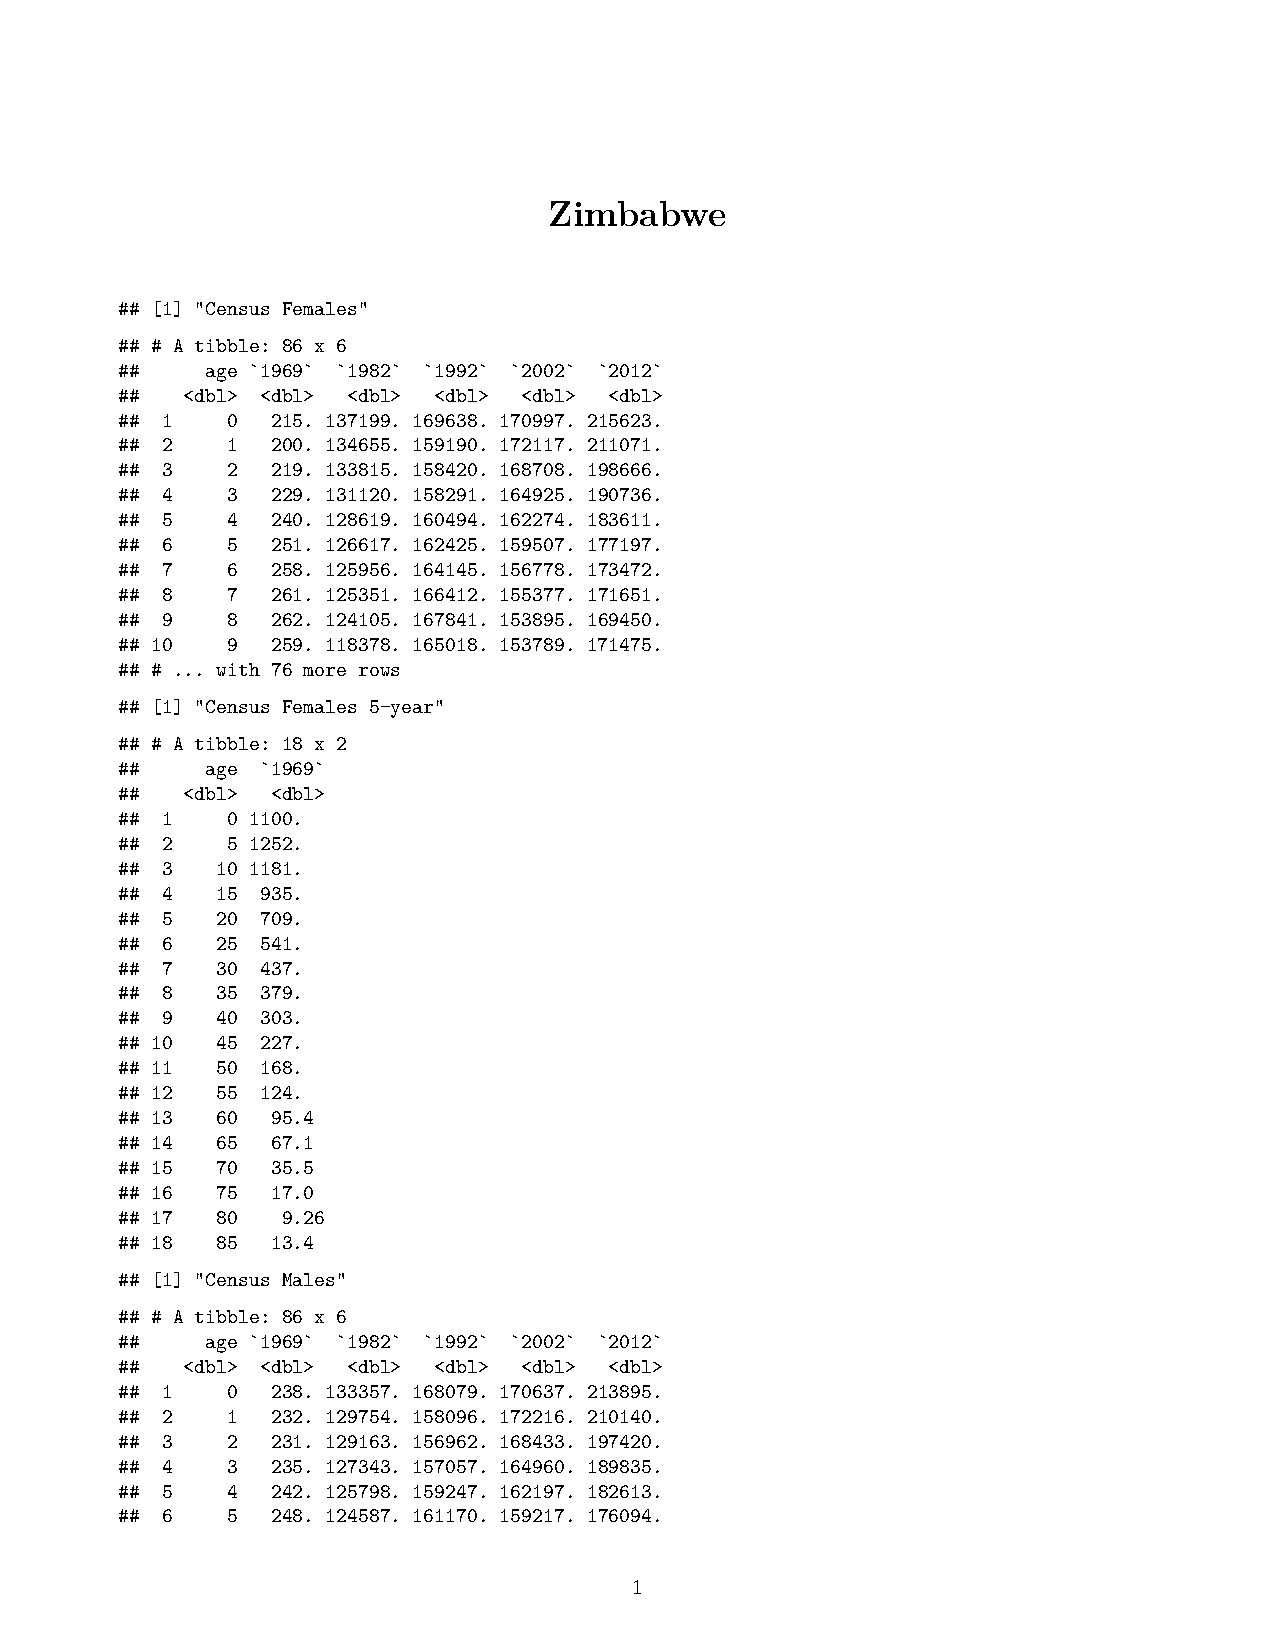
\includepdf[pages=-]{"../thiele_RW_Gumbel_reports/Zimbabwe P2.pdf"}

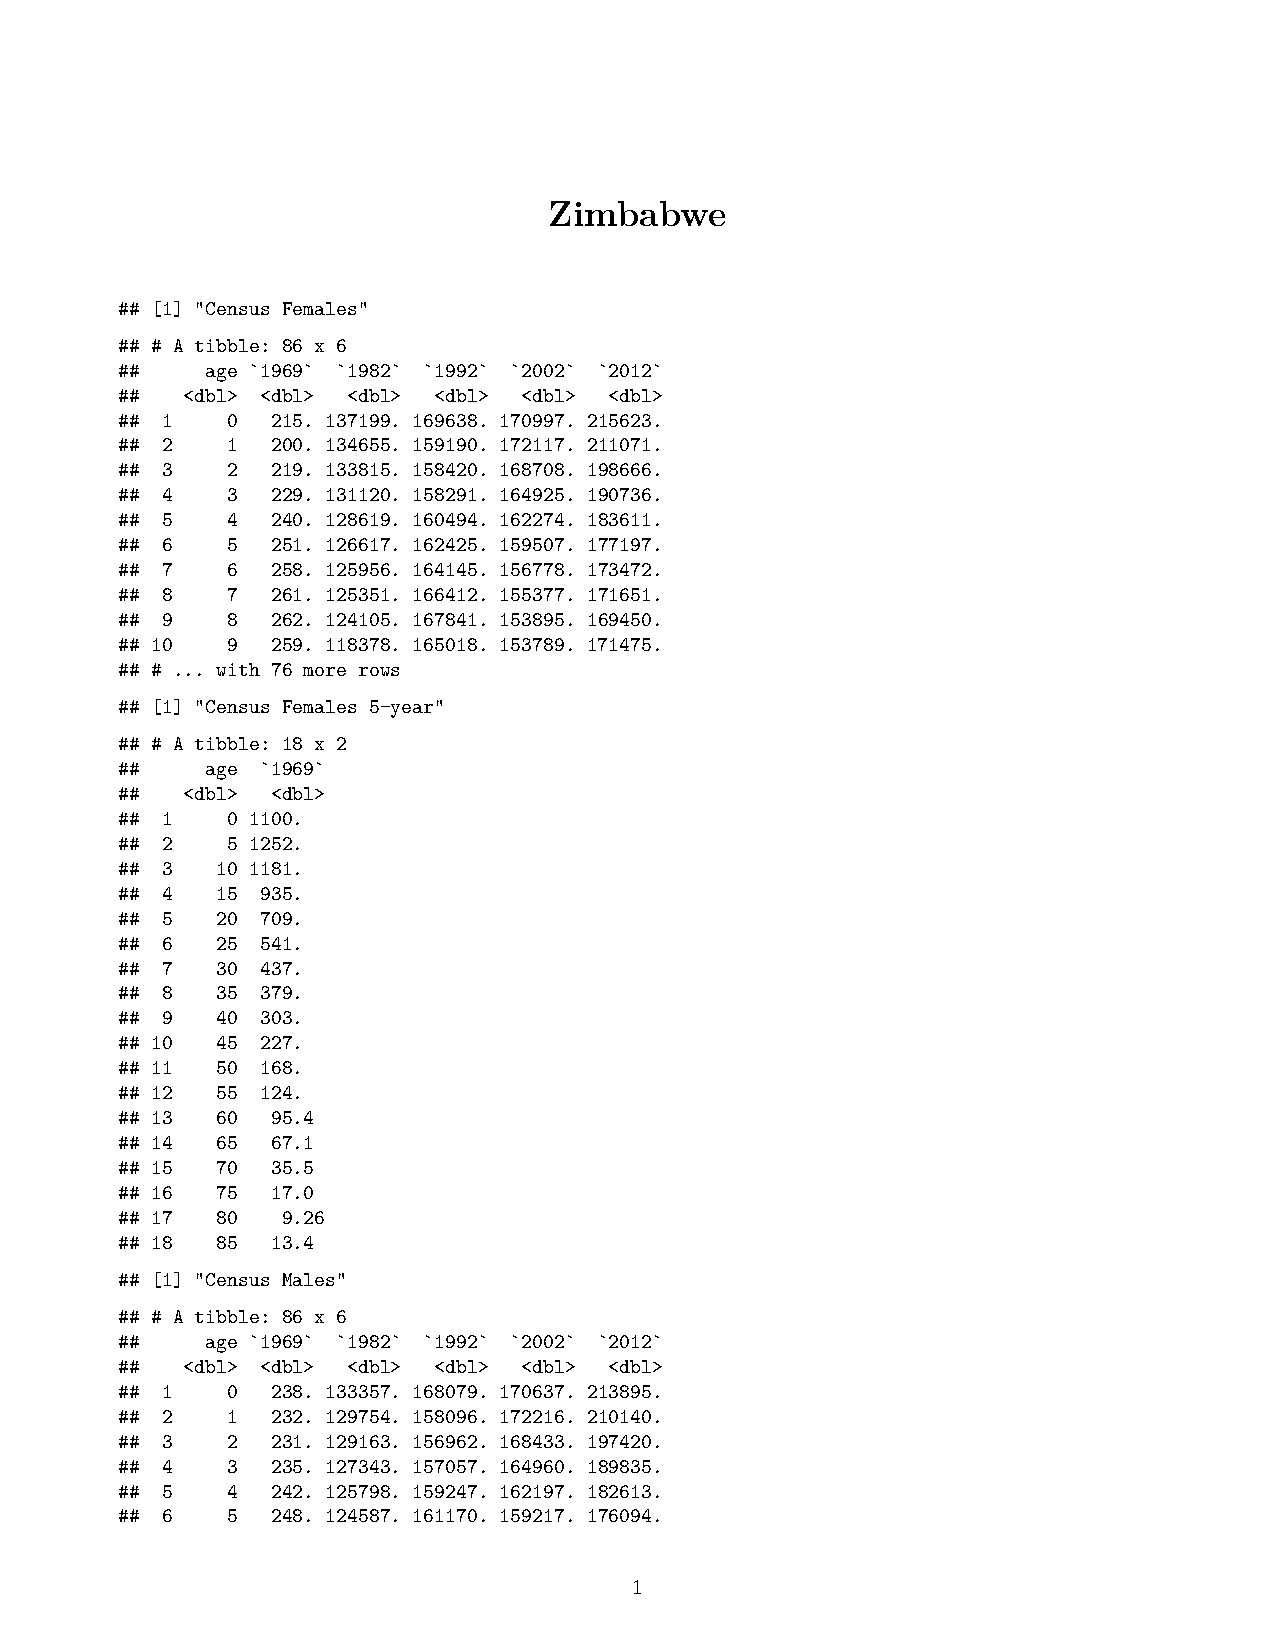
\includepdf[pages=-]{"../thiele_RW_Gumbel_reports/Zimbabwe P1.pdf"}

\end{document}